\documentclass[14pt,a4paper]{extreport}
% -------------------- Кодировка и язык --------------------
\usepackage[T2A]{fontenc}
\usepackage[utf8]{inputenc}
\usepackage[russian]{babel}
% -------------------- Поля страницы (А4, переплет) --------------------
\usepackage{geometry}
\geometry{
    a4paper,
    left=30mm,
    right=15mm,
    top=20mm,
    bottom=20mm
}
% -------------------- Межстрочный интервал и абзац --------------------
\usepackage{setspace}
\onehalfspacing
\usepackage{indentfirst}
\setlength{\parindent}{1.25cm}
% -------------------- Выравнивание по ширине --------------------
\usepackage{ragged2e}
% -------------------- Математика, рисунки, таблицы --------------------
\usepackage{amsmath,amssymb}
\usepackage{graphicx}
\usepackage{float}
\usepackage{caption}
\usepackage{booktabs}
\usepackage{array}
\usepackage{longtable}
\usepackage{tabularx}
\usepackage{multirow}
% -------------------- Оглавление и заголовки --------------------
\usepackage{titlesec}
\usepackage{tocloft}
\titleformat{\chapter}[block]
    {\normalfont\bfseries\centering}
    {\thechapter}
    {1em}
    {\MakeUppercase}
\titleformat{\section}
    {\normalfont\bfseries}
    {\thesection}
    {1em}
    {}
\titleformat{\subsection}
    {\normalfont\bfseries}
    {\thesubsection}
    {1em}
    {}
% -------------------- Колонтитулы --------------------
\usepackage{fancyhdr}
\pagestyle{fancy}
\fancyhf{}
\fancyfoot[C]{\thepage}
\renewcommand{\headrulewidth}{0pt}
% -------------------- Гиперссылки --------------------
\usepackage[hidelinks]{hyperref}
% -------------------- Названия --------------------
\addto\captionsrussian{
    \renewcommand{\contentsname}{СОДЕРЖАНИЕ}
    \renewcommand{\chaptername}{Глава}
    \renewcommand{\bibname}{СПИСОК ИСПОЛЬЗОВАННЫХ ИСТОЧНИКОВ}
}
\begin{document}
\justifying
% ==================== ТИТУЛЬНЫЙ ЛИСТ ====================
\begin{titlepage}
    \begin{center}
        Министерство науки и высшего образования Российской Федерации\\[0.5cm]
        Федеральное государственное автономное образовательное учреждение высшего образования\\[0.3cm]
        \textbf{«Московский физико-технический институт\\
        (национальный исследовательский университет)»}\\[1.5cm]
        Кафедра \rule{9cm}{0.4pt}\\[0.5cm]
        Направление подготовки \rule{6cm}{0.4pt}\\[2cm]
        {\bfseries\large ВЫПУСКНАЯ КВАЛИФИКАЦИОННАЯ РАБОТА}\\[0.5cm]
        {\bfseries\large (ДИПЛОМНАЯ РАБОТА)}\\[1.5cm]
        {\bfseries\Large Автоматический перевод\\
        и распознавание рунических текстов}
    \end{center}
\end{titlepage}
\newpage
\pagenumbering{arabic}
% ==================== СОДЕРЖАНИЕ ====================
\tableofcontents
\newpage
% ==================== ВВЕДЕНИЕ ====================
\chapter*{Аннотация}
\addcontentsline{toc}{chapter}{Аннотация}
Текст введения.
\textbf{Актуальность темы.} \\
Текст введения.

% ==================== ГЛАВА 1 ====================
\chapter{ВВЕДЕНИЕ}
\section{История и лингвистические особенности рунической письменности}
Текст раздела.

% ==================== ГЛАВА 2 ====================
\chapter{ОБЗОР ЛИТЕРАТУРЫ}
\section{Обзор литературы}
Текст раздела.

% ==================== ГЛАВА 3 ====================
\chapter{ДАННЫЕ}

Качество обучения моделей машинного обучения в значительной степени определяется качеством и объёмом данных. В задачах перевода рунических текстов проблема формирования корпуса параллельного перевода является одной из основных в силу ограниченного числа сохранившихся рунических текстов.

\section{Источники данных}

Для формирования корпуса были использованы следующие источники:

\begin{enumerate}
    \item \textbf{Открытые базы рунических надписей.} Основным источником послужила база данных Rundata~\cite{rundata}, содержащая транслитерации и переводы свыше 6500 скандинавских рунических надписей и текстов

    \item \textbf{Сайт с фотографиями RuneS.} Второй источник -- сайт RuneS ~\cite{runes}, включающий в себя около 8100 фотографий вместе с транслитерацией древнескандинавских рунических надписей. В основном надписи находятся на камнях и древних орудиях труда. Особенностью данных с этого сайта это наличие датировки данных.

    \item \textbf{Сайт с фотографиями christerhamp.} Третий источник по объёму сайт christerhamp ~\cite{christerhamp}, содержащий чуть больше 3000 изображений с транслитерацией рунических надписей.
    
\end{enumerate}


\section{Предобработка текстов}

Для задачи перевода применялась следующая текстовая предобработка:

\begin{enumerate}
    \item \textbf{Нормализация рунического текста.} Все рунические надписи приводились к единому формату:
    \begin{itemize}
        \item Удаление специальных символов разметки (¶, •, ·), не несущих лингвистической нагрузки.
        \item Замена специфических символов на стандартные латинские аналоги (например, þ $\to$ th, ð $\to$ d, æ $\to$ ae).
        \item Приведение к нижнему регистру для унификации.
        \item Удаление лишних пробелов и нормализация пробельных символов.
    \end{itemize}
    
    \item \textbf{Обработка пропусков и повреждений.} В случае повреждённых или нечитаемых участков текста:
    \begin{itemize}
        \item Пропуски обозначались специальным токеном \texttt{[UNK]}.
        \item Частично сохранившиеся слова маркировались символом \texttt{*}.
        \item Реконструированные фрагменты заключались в квадратные скобки \texttt{[]}.
    \end{itemize}
    
    \item \textbf{Токенизация переводов.} Для современных языков (английский, немецкий, шведский):
    \begin{itemize}
        \item Использование стандартных токенизаторов моделей (Qwen Tokenizer, Gemma Tokenizer).
        \item Сохранение пунктуации как отдельных токенов.
        \item Обработка составных слов (особенно для немецкого языка).
    \end{itemize}
    
    \item \textbf{Фильтрация данных.} Исключение некорректных примеров:
    \begin{itemize}
        \item Удаление пар с пустыми или слишком короткими переводами (< 3 слов).
        \item Исключение дубликатов.
        \item Проверка соответствия языка перевода целевому языку.
    \end{itemize}
\end{enumerate}

\section{Корпус для задачи перевода}

Для задачи машинного перевода был собран параллельный корпус, содержащий транслитерации рунических надписей (в латинской нотации) и их переводы на современные языки (английский, немецкий, шведский). Характеристики корпуса представлены в таблице~\ref{tab:mt_data}.

\begin{table}[H]
\centering
\caption{Характеристика параллельного корпуса для задачи перевода}
\label{tab:mt_data}
\begin{tabular}{|l|c|}
\hline
\textbf{Языковая пара} & \textbf{Пар предложений}\\
\hline
Руническая транслитерация $\to$ английский & 3662 \\
\hline
Руническая транслитерация $\to$ немецкий & 2766 \\
\hline
Руническая транслитерация $\to$ шведский & 1875 \\
\hline
\textbf{Итого} & \textbf{8203} \\
\hline
\end{tabular}
\end{table}

\section{Разделение выборки}

Корпус был разделён на обучающую, валидационную и тестовую выборки в соотношении 80:10:10. Такое разделение является стандартным в задачах машинного обучения и позволяет:

\begin{itemize}
    \item \textbf{Обучающая выборка (80\%).} Используется для непосредственного обучения модели. На этих данных модель корректирует свои веса в процессе градиентного спуска.
    
    \item \textbf{Валидационная выборка (10\%).} Применяется для подбора гиперпараметров и ранней остановки обучения (early stopping). Модель не обучается на этих данных, но они используются для оценки качества в процессе обучения.
    
    \item \textbf{Тестовая выборка (10\%).} Служит для финальной оценки качества обученной модели. Эти данные не используются ни на одном из этапов обучения или подбора параметров.
\end{itemize}

Разделение производилось стратифицированно по языкам, чтобы сохранить пропорции языковых пар во всех выборках. Данные перемешивались случайным образом перед разделением для исключения систематических смещений.

\begin{table}[H]
\centering
\caption{Распределение данных по выборкам}
\label{tab:split}
\begin{tabular}{|l|c|c|c|c|}
\hline
\textbf{Языковая пара} & \textbf{Всего} & \textbf{Обучающая} & \textbf{Валидационная} & \textbf{Тестовая} \\
\hline
Руническая $\to$ английский & 3662 & 2930 & 366 & 366 \\
\hline
Руническая $\to$ немецкий & 2766 & 2213 & 277 & 276 \\
\hline
Руническая $\to$ шведский & 1875 & 1500 & 188 & 187 \\
\hline
\textbf{Итого} & \textbf{8203} & \textbf{6643} & \textbf{831} & \textbf{829} \\
\hline
\end{tabular}
\end{table}

Для обеспечения воспроизводимости результатов использовался фиксированный параметр случайной генерации (random seed = 42) при разделении данных.

\section{Данные для предсказания датировки надписей}

Помимо задачи машинного перевода, в рамках данного исследования решалась задача предсказания датировки рунических надписей. Для этой задачи был собран отдельный корпус данных, содержащий транслитерации надписей и их предполагаемые даты создания.

\subsection{Источники данных для датировки}

Основным источником данных для задачи датировки послужил сайт RuneS~\cite{runes}, содержащий информацию о датировке рунических надписей. В отличие от других источников, RuneS предоставляет датировку в явном виде, что делает его ценным ресурсом для обучения моделей регрессии.

\begin{table}[H]
\centering
\caption{Характеристика корпуса для задачи датировки}
\label{tab:dating_data}
\begin{tabular}{|l|c|}
\hline
\textbf{Параметр} & \textbf{Значение} \\
\hline
Общее количество надписей с датировкой & 1247 \\
\hline
Диапазон дат & 500--1500 гг. н.э. \\
\hline
Средняя длина надписи (токенов) & 45 \\
\hline
Минимальная длина надписи & 5 токенов \\
\hline
Максимальная длина надписи & 312 токенов \\
\hline
\end{tabular}
\end{table}

\subsection{Формат представления дат}

Датировка надписей представлена в следующем формате:
\begin{itemize}
    \item \textbf{Точные даты.} Для некоторых надписей известна точная дата создания (например, «1050 год»).
    \item \textbf{Диапазоны дат.} Для большинства надписей датировка представлена в виде диапазона (например, «1000--1050 гг.»).
    \item \textbf{Приблизительные даты.} Часть надписей имеет приблизительную датировку (например, «конец X века», «первая половина XI века»).
\end{itemize}

Для обучения модели датировки все даты были преобразованы в числовой формат — количество лет от начала нашей эры. Для диапазонов дат использовалось среднее значение.

\subsection{Предобработка данных для датировки}

Для задачи предсказания датировки применялась следующая предобработка:

\begin{enumerate}
    \item \textbf{Фильтрация по качеству датировки.} Исключены надписи с неопределённой датировкой (например, «средневековье», «древность»).
    
    \item \textbf{Нормализация текста.} Аналогично задаче перевода: удаление специальных символов, приведение к нижнему регистру, нормализация пробелов.
    
    \item \textbf{Балансировка по векам.} Данные сбалансированы таким образом, чтобы каждый век был представлен примерно одинаковым количеством примеров. Это необходимо для предотвращения смещения модели в сторону более частых периодов.
    
    \item \textbf{Аугментация данных.} Для увеличения размера выборки применены методы аугментации:
    \begin{itemize}
        \item Синонимическая замена распространённых слов.
        \item Случайное удаление неключевых токенов (с вероятностью 0.1).
        \item Перестановка соседних слов (с вероятностью 0.05).
    \end{itemize}
\end{enumerate}

\subsection{Разделение выборки для датировки}

Корпус для задачи датировки был разделён на обучающую, валидационную и тестовую выборки в соотношении 80:10:10. Разделение производилось стратифицированно по векам для сохранения распределения дат во всех выборках.

\begin{table}[H]
\centering
\caption{Распределение данных для датировки по выборкам}
\label{tab:dating_split}
\begin{tabular}{|l|c|c|c|}
\hline
\textbf{Выборка} & \textbf{Количество} & \textbf{Доля} & \textbf{Диапазон дат} \\
\hline
Обучающая & 998 & 80\% & 500--1500 гг. \\
\hline
Валидационная & 125 & 10\% & 550--1450 гг. \\
\hline
Тестовая & 124 & 10\% & 600--1400 гг. \\
\hline
\textbf{Итого} & \textbf{1247} & \textbf{100\%} & \textbf{500--1500 гг.} \\
\hline
\end{tabular}
\end{table}

\subsection{Распределение надписей по векам}

На рисунке~\ref{fig:dating_distribution} представлено распределение надписей по векам. Как видно из графика, наибольшее количество надписей приходится на XI--XII века, что соответствует периоду расцвета рунической традиции в Скандинавии.

\begin{figure}[H]
\centering
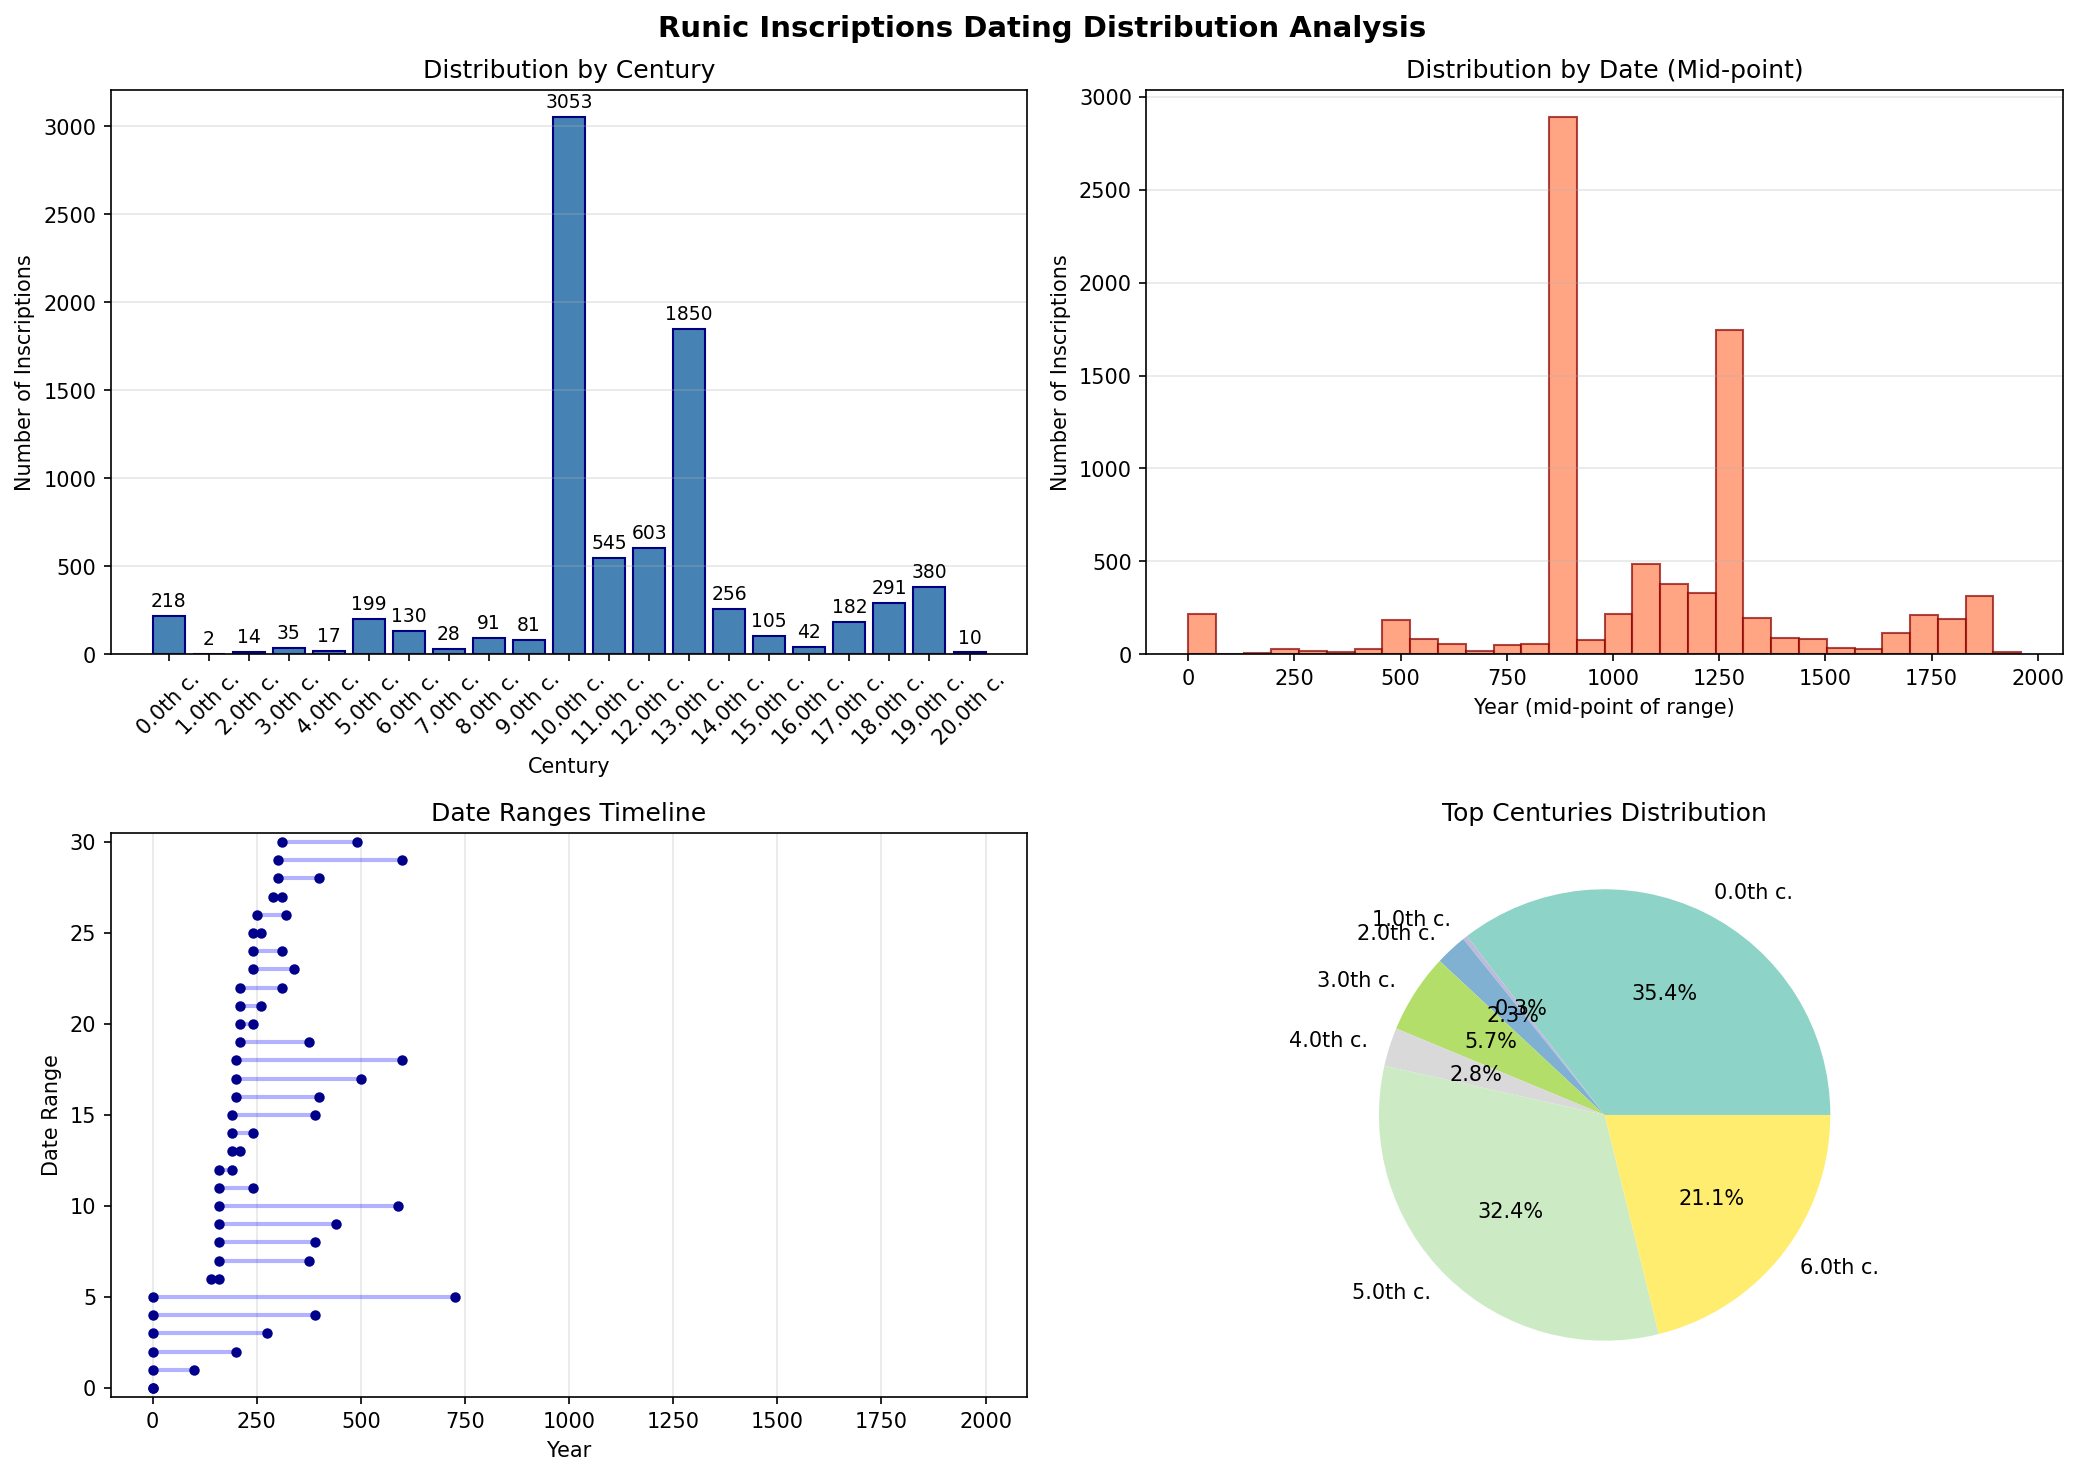
\includegraphics[width=0.8\textwidth]{plots/dating_distribution_analysis.png}
\caption{Распределение рунических надписей по векам}
\label{fig:dating_distribution}
\end{figure}

\textbf{Наблюдения:}
\begin{itemize}
    \item Пик количества надписей приходится на XI век (около 400 надписей).
    \item Надписи X и XV веков представлены наименьшим количеством примеров.
    \item Распределение имеет правостороннюю асимметрию, что характерно для исторических данных.
\end{itemize}

\section{Проблемы и ограничения корпуса}

В процессе формирования корпуса данных были выявлены следующие проблемы:
\begin{itemize}
    \item \textbf{Повреждения и утраты.} Значительная часть надписей имеет пропуски и пробелы. Большинство предложений имеют пропуски в середине, упущены некоторые слова. Также некоторые слова имеют неоднозначно распознанные символы.
    
    \item \textbf{Неточность датировки.} Для многих надписей датировка является приблизительной и основана на стилистических особенностях, а не на археологических данных.
    
    \item \textbf{Дисбаланс по периодам.} Надписи распределены неравномерно по векам, что может привести к смещению модели в сторону более частых периодов.
    
    \item \textbf{Ограниченный размер выборки.} Общее количество надписей с надёжной датировкой (1247) является относительно небольшим для обучения глубоких моделей.
\end{itemize}

\section*{Выводы}
\addcontentsline{toc}{section}{Выводы}



% ==================== ГЛАВА 4 ====================
\chapter{МЕТОДЫ}

\section{Метрики качества перевода}
Оценка качества машинного перевода имеет большое значение при обучении моделей. Чтобы численно определить, насколько компьютерный перевод близок к тому, что сделал бы человек в качестве эталона, существуют обещепринятые метрики качества перевода. Опираясь на эти метрики мы будем оценивать насколько хорошую модель мы получили. Далее описаны некоторые из популярных метрик, которые я использовал для оценок своих моделей: BLEU, chrF, chrF++, METEOR. Каждая из этих метрик основывается на совпадениях $n$-грамм, но учитывает их по-своему.

\subsection{Метрика BLEU}

Метрика \textbf{BLEU} (Bilingual Evaluation Understudy) была предложена Папинени и соавторами в 2002 году \cite{papineni2002bleu} и на сегодняшний день является наиболее широко используемой метрикой  оценки качества машинного перевода. В основе метрики лежит идея измерения степени совпадения $n$-грамм в гипотезе перевода и одном или нескольких эталонных переводах.

Для каждого порядка $n$ вычисляется модифицированная точность (modified $n$-gram precision):
\begin{equation}
p_n = \frac{\sum_{C \in \{Candidates\}} \sum_{n\text{-gram} \in C} \mathrm{Count}_{clip}(n\text{-gram})}{\sum_{C' \in \{Candidates\}} \sum_{n\text{-gram}' \in C'} \mathrm{Count}(n\text{-gram}')},
\end{equation}
где $\mathrm{Count}_{clip}$~--- это <<обрезанное>> число вхождений $n$-граммы, ограниченное максимальным числом её вхождений в любом из эталонных переводов. Такое обрезание предотвращает искусственное завышение оценки за счёт многократного повторения частых слов.

Итоговое значение BLEU вычисляется как геометрическое среднее модифицированных точностей для $n$-грамм порядка от 1 до $N$ (обычно $N = 4$), умноженное на штраф за краткость (brevity penalty, $BP$):
\begin{equation}
\mathrm{BLEU} = BP \cdot \exp\left(\sum_{n=1}^{N} w_n \log p_n\right),
\end{equation}
где $w_n = 1/N$~--- весовые коэффициенты, а штраф за краткость определяется как:
\begin{equation}
BP =
\begin{cases}
1, & \text{если } c > r, \\
\exp\left(1 - r/c\right), & \text{если } c \leq r,
\end{cases}
\end{equation}
где $c$~--- суммарная длина гипотезы перевода, $r$~--- длина ближайшего по длине эталонного перевода. Штраф за краткость необходим, поскольку метрика точности не учитывает полноту перевода: без него короткие переводы получали бы необоснованно высокие оценки.

Значение BLEU лежит в диапазоне $[0, 1]$ (часто умножается на 100), причём большее значение соответствует лучшему качеству. Основными недостатками BLEU являются: работа на уровне точных совпадений слов (без учёта синонимов и морфологических форм), слабая корреляция с человеческой оценкой на уровне отдельных предложений, а также низкая информативность для морфологически богатых языков.

\subsection{Метрика chrF}

Метрика \textbf{chrF} (character $n$-gram F-score), предложенная М.~Поповичем в 2015 году \cite{popovic2015chrf}, основана на $F$-мере, вычисляемой по $n$-граммам символов, а не слов. Такой подход позволяет лучше учитывать морфологические особенности языков и частичные совпадения словоформ, что особенно важно для флективных и агглютинативных языков.


Пусть $\mathrm{chrP}_n$ и $\mathrm{chrR}_n$~--- точность и полнота для символьных $n$-грамм порядка $n$:
\begin{equation}
\mathrm{chrP}_n = \frac{\text{число совпадающих } n\text{-грамм}}{\text{общее число } n\text{-грамм в гипотезе}},
\end{equation}
\begin{equation}
\mathrm{chrR}_n = \frac{\text{число совпадающих } n\text{-грамм}}{\text{общее число } n\text{-грамм в эталоне}}.
\end{equation}


Итоговая оценка chrF определяется как $F_\beta$-мера, усреднённая по $n$-граммам от 1 до $N$ (обычно $N = 6$):
\begin{equation}
\mathrm{chrF}_\beta = (1 + \beta^2) \cdot \frac{\mathrm{chrP} \cdot \mathrm{chrR}}{\beta^2 \cdot \mathrm{chrP} + \mathrm{chrR}},
\end{equation}
где $\mathrm{chrP}$ и $\mathrm{chrR}$~--- усреднённые по всем $n$ значения точности и полноты, а параметр $\beta$ регулирует относительную важность полноты по отношению к точности. При $\beta = 1$ метрика называется \textbf{chrF1} и придаёт точности и полноте равный вес, при $\beta = 2$~--- \textbf{chrF2}, где полнота в два раза важнее точности.


Метрика chrF не зависит от токенизатора, что делает её применимой к любым языкам, включая те, в которых отсутствуют явные разделители слов. Эмпирические исследования показывают более высокую корреляцию chrF с человеческими оценками по сравнению с BLEU, особенно на уровне отдельных сегментов текста.

\subsection{Метрика chrF++}

Метрика \textbf{chrF++} является расширением chrF, предложенным тем же автором в 2017 году \cite{popovic2017chrf}. Основное отличие заключается в том, что помимо символьных $n$-грамм в расчёт включаются также словесные $n$-граммы низких порядков (обычно униграммы и биграммы слов).


Формула аналогична chrF, но точность и полнота вычисляются как среднее значений, полученных для символьных $n$-грамм порядков от 1 до $N$ (по умолчанию $N = 6$) и словесных $n$-грамм порядков от 1 до $M$ (по умолчанию $M = 2$):
\begin{equation}
\mathrm{chrF{+}{+}} = (1 + \beta^2) \cdot \frac{\overline{P} \cdot \overline{R}}{\beta^2 \cdot \overline{P} + \overline{R}},
\end{equation}
где $\overline{P}$ и $\overline{R}$~--- усреднённые по всем выбранным $n$-граммам (как символьным, так и словесным) значения точности и полноты.


Добавление словесных $n$-грамм позволяет метрике лучше учитывать порядок слов и синтаксические соответствия, сохраняя при этом преимущества символьного подхода. Согласно результатам конференций WMT, chrF++ демонстрирует более высокую корреляцию с человеческими оценками качества по сравнению как с BLEU, так и с исходной chrF, и рекомендуется в качестве одной из основных метрик для оценки машинного перевода.

\subsection{Метрика METEOR}

Метрика \textbf{METEOR} (Metric for Evaluation of Translation with Explicit ORdering) была предложена Банерджи и Лави в 2005 году \cite{banerjee2005meteor} как альтернатива BLEU, призванная устранить ряд её недостатков. Ключевыми особенностями METEOR являются: использование взвешенной $F$-меры с приоритетом полноты, учёт синонимов и морфологических форм, а также явный штраф за нарушение порядка слов.


Построение соответствия между словами гипотезы и эталонного перевода (alignment) производится в несколько этапов:
\begin{enumerate}
    \item \textbf{Точное совпадение} (exact match)~--- совпадение словоформ;
    \item \textbf{Стемминг} (stem match)~--- совпадение основ слов после морфологической нормализации;
    \item \textbf{Синонимическое совпадение} (synonym match)~--- совпадение через словарь синонимов (например, WordNet);
    \item \textbf{Парафразное совпадение} (paraphrase match)~--- совпадение через базу парафраз (в поздних версиях METEOR~1.5).
\end{enumerate}


На основе построенного соответствия вычисляются точность $P$ и полнота $R$:
\begin{equation}
P = \frac{m}{w_c}, \quad R = \frac{m}{w_r},
\end{equation}
где $m$~--- число слов гипотезы, сопоставленных со словами эталона, $w_c$ и $w_r$~--- число слов в гипотезе и эталоне соответственно.

Далее вычисляется гармоническое среднее $F_{mean}$ с приоритетом полноты:
\begin{equation}
F_{mean} = \frac{P \cdot R}{\alpha \cdot P + (1 - \alpha) \cdot R},
\end{equation}
где параметр $\alpha$ (обычно $\alpha = 0.9$) задаёт относительный вес точности и полноты.
Для учёта порядка слов вводится штраф за фрагментацию (fragmentation penalty):

\begin{equation}
\mathrm{Penalty} = \gamma \cdot \left(\frac{ch}{m}\right)^\theta,
\end{equation}
где $ch$~--- число <<кусков>> (chunks), то есть максимальных непрерывных последовательностей слов, совпадающих в гипотезе и эталоне в одинаковом порядке; $\gamma$ и $\theta$~--- настраиваемые параметры (обычно $\gamma = 0.5$, $\theta = 3$). Чем больше число фрагментов при том же количестве совпадений, тем сильнее нарушен порядок слов и тем выше штраф.

Итоговое значение метрики вычисляется по формуле:
\begin{equation}
\mathrm{METEOR} = F_{mean} \cdot (1 - \mathrm{Penalty}).
\end{equation}


Метрика METEOR демонстрирует более высокую корреляцию с человеческими оценками качества на уровне отдельных предложений по сравнению с BLEU. К её преимуществам относятся учёт лингвистических знаний (морфология, синонимия) и явное моделирование порядка слов. Основными недостатками являются зависимость от внешних ресурсов (словарей синонимов, стеммеров), что ограничивает применение METEOR для малоресурсных языков, а также более высокая вычислительная сложность.

\section{Модели для обучения и методы обучения}

В рамках данного исследования были использованы современные архитектуры больших языковых моделей (Large Language Models, LLM), основанные на трансформере. Выбор конкретных моделей обусловлен их открытой лицензией, доступностью весов и архитектурными особенностями, подходящими для задачи машинного перевода рунических текстов.

\subsection{Архитектура трансформера}

Основой всех использованных моделей служит архитектура трансформера, предложенная в работе \cite{vaswani2017attention}. Ключевыми компонентами трансформера являются:

\begin{itemize}
    \item \textbf{Механизм самовнимания (Self-Attention).} Позволяет модели учитывать контекст всех слов в последовательности при кодировании каждого отдельного слова. Для входной последовательности длины $n$ механизм внимания вычисляет взвешенную сумму значений:
    \begin{equation}
    \mathrm{Attention}(Q, K, V) = \mathrm{softmax}\left(\frac{QK^T}{\sqrt{d_k}}\right)V,
    \end{equation}
    где $Q$, $K$, $V$~--- матрицы запросов, ключей и значений соответственно, $d_k$~--- размерность ключей.
    
    \item \textbf{Позиционное кодирование.} Поскольку трансформер не имеет встроенного представления о порядке элементов, позиционная информация добавляется через специальные кодировки:
    \begin{equation}
    PE_{(pos, 2i)} = \sin\left(\frac{pos}{10000^{2i/d_{model}}}\right), \quad
    PE_{(pos, 2i+1)} = \cos\left(\frac{pos}{10000^{2i/d_{model}}}\right).
    \end{equation}
    
    \item \textbf{Многослойные перцептроны (Feed-Forward Networks).} Применяются независимо к каждой позиции после механизма внимания.
\end{itemize}

\subsection{Модель Qwen3.5}

Семейство моделей Qwen3.5 представляет собой современные декодерные языковые модели с архитектурой, оптимизированной для эффективной работы с длинными последовательностями. В исследовании использовались модели следующих размеров:

\begin{itemize}
    \item \textbf{Qwen3.5-0.8B}~--- 0.8 миллиарда параметров, базовая модель для экспериментов с дообучением.
    \item \textbf{Qwen3.5-2B}~--- 2 миллиарда параметров, промежуточный размер для анализа масштабирования.
    \item \textbf{Qwen3.5-4B}~--- 4 миллиарда параметров, оптимальный баланс между качеством и вычислительными затратами.
    \item \textbf{Qwen3.5-9B}~--- 9 миллиардов параметров, наибольшая модель для оценки предельного качества.
\end{itemize}

Архитектурные особенности Qwen3.5:
\begin{itemize}
    \item Использование группированных запросов внимания (Grouped Query Attention, GQA) для ускорения инференса.
    \item Скользящее окно внимания (Sliding Window Attention) для эффективной работы с длинным контекстом.
    \item Функция активации SwiGLU с расширенным промежуточным слоем.
    \item Нормализация RMSNorm вместо стандартной LayerNorm.
\end{itemize}

\subsection{Модель Gemma-2-2B}

Модель Gemma-2-2B от Google представляет собой облегчённую версию семейства Gemma, оптимизированную для эффективного развёртывания. Архитектурные особенности:

\begin{itemize}
    \item 2 миллиарда параметров при высокой плотности знаний.
    \item Локальное внимание с окном 4096 токенов.
    \item Мягкое введение (soft introduction) для улучшения сходимости при обучении.
    \item Интеграция с экосистемой Hugging Face и JAX/Flax.
\end{itemize}

\subsection{Метод дообучения LoRA}

Для адаптации предобученных моделей к задаче перевода рунических текстов использовался метод Low-Rank Adaptation (LoRA) \cite{hu2021lora}. Основная идея LoRA заключается в замораживании весов предобученной модели и добавлении обучаемых низкоранговых матриц.

Формально, для матрицы весов $W_0 \in \mathbb{R}^{d \times k}$ предобученной модели, обновление представляется как:
\begin{equation}
W = W_0 + \Delta W = W_0 + BA,
\end{equation}
где $B \in \mathbb{R}^{d \times r}$, $A \in \mathbb{R}^{r \times k}$~--- обучаемые матрицы низкого ранга $r \ll \min(d, k)$.

Преимущества LoRA:
\begin{itemize}
    \item \textbf{Эффективность памяти.} Обучаются только 0.1--1\% параметров модели, что позволяет дообучать большие модели на ограниченном оборудовании.
    \item \textbf{Отсутствие задержки инференса.} После обучения матрицы $A$ и $B$ могут быть объединены с $W_0$, не добавляя вычислительных затрат.
    \item \textbf{Модульность.} Для разных задач можно обучать отдельные адаптеры LoRA и переключаться между ними без изменения базовой модели.
\end{itemize}

В данном исследовании использовались следующие гиперпараметры LoRA:
\begin{itemize}
    \item Ранг адаптера: $r = 16$
    \item Масштабирование: $\alpha = 32$
    \item Применяемые модули: attention query и value проекции
    \item Dropout: 0.05
\end{itemize}

\subsection{Процесс дообучения}

Дообучение моделей осуществлялось в несколько этапов:

\begin{enumerate}
    \item \textbf{Подготовка данных.} Параллельный корпус был разделён на обучающую (80\%), валидационную (10\%) и тестовую (10\%) выборки.
    
    \item \textbf{Токенизация.} Использовался родной токенизатор каждой модели для преобразования текста в последовательности токенов.
    
    \item \textbf{Обучение.} Модель обучалась с использованием функции потерь кросс-энтропии:
    \begin{equation}
    \mathcal{L} = -\sum_{t=1}^{T} \log P(y_t | y_{<t}, x),
    \end{equation}
    где $x$~--- исходная последовательность (рунический текст), $y$~--- целевая последовательность (перевод).
    
    \item \textbf{Валидация.} После каждой эпохи оценивалось качество на валидационной выборке с использованием метрик BLEU и chrF++.
    
    \item \textbf{Сохранение адаптеров.} Сохранялись только веса адаптеров LoRA, что позволяло эффективно хранить множество специализированных моделей.
\end{enumerate}

\subsection{Гиперпараметры обучения}

В таблице~\ref{tab:training_params} представлены гиперпараметры, использованные при дообучении моделей.

\begin{table}[H]
\centering
\caption{Гиперпараметры дообучения моделей}
\label{tab:training_params}
\begin{tabular}{|l|c|}
\hline
\textbf{Параметр} & \textbf{Значение} \\
\hline
Размер пакета (batch size) & 16 \\
\hline
Скорость обучения (learning rate) & $2 \times 10^{-4}$ \\
\hline
Количество эпох & 20 \\
\hline
Ранг LoRA ($r$) & 16 \\
\hline
Масштаб LoRA ($\alpha$) & 32 \\
\hline
Dropout & 0.05 \\
\hline
Оптимизатор & AdamW \\
\hline
Планировщик скорости обучения & Cosine decay \\
\hline
Максимальная длина последовательности & 512 \\
\hline
\end{tabular}
\end{table}

\section{Данные для обучения}

Для обучения моделей использовался параллельный корпус рунических текстов, описанный в главе~3. Корпус содержит 8203 пары «руническая транслитерация~--- перевод» на трёх языках: английском, немецком и шведском.

% ==================== ГЛАВА 5 ====================
\chapter{РЕЗУЛЬТАТЫ}
\section{Метрики качества перевода}

Для оценки качества моделей были использованы метрики BLEU и chrF++. В данном разделе представлены результаты оценки всех протестированных моделей до и после дообучения.

\subsection{Метрики базовых моделей}

В таблице~\ref{tab:base_metrics} представлены метрики качества для базовых моделей Qwen3.5 различных размеров (0.8B, 2B, 4B, 9B параметров) на трёх языках.

\begin{table}[H]
\centering
\caption{Метрики качества базовых моделей Qwen3.5}
\label{tab:base_metrics}
\begin{tabular}{|l|l|c|c|}
\hline
\textbf{Модель} & \textbf{Язык} & \textbf{BLEU} & \textbf{chrF++} \\
\hline
\multirow{3}{*}{\texttt{Qwen3.5-0.8B}} & Английский & 2.31 & 11.82 \\
\cline{2-4}
& Немецкий & 1.55 & 9.99 \\
\cline{2-4}
& Шведский & 0.35 & 10.60 \\
\hline
\multirow{3}{*}{\texttt{Qwen3.5-2B}} & Английский & 4.32 & 13.81 \\
\cline{2-4}
& Немецкий & 3.96 & 11.08 \\
\cline{2-4}
& Шведский & 0.69 & 12.21 \\
\hline
\multirow{3}{*}{\texttt{Qwen3.5-4B}} & Английский & 4.52 & 15.61 \\
\cline{2-4}
& Немецкий & 5.79 & 11.61 \\
\cline{2-4}
& Шведский & 0.79 & 9.69 \\
\hline
\multirow{3}{*}{\texttt{Qwen3.5-9B}} & Английский & 4.21 & 17.89 \\
\cline{2-4}
& Немецкий & 2.96 & 12.32 \\
\cline{2-4}
& Шведский & 2.67 & 16.17 \\
\hline
\end{tabular}
\end{table}

\textbf{Наблюдения:}
\begin{itemize}
    \item \textbf{Английский язык} показывает наилучшие результаты среди всех языков для базовых моделей, что объясняется большим объёмом англоязычных данных в предобучении.
    \item \textbf{Модель 9B} демонстрирует лучшие результаты по метрике chrF++ для английского (17.89) и шведского (16.17) языков, что указывает на лучшее понимание морфологической структуры.
    \item \textbf{Немецкий язык} показывает промежуточные результаты, при этом модель 4B достигает наилучшего BLEU (5.79).
    \item \textbf{Шведский язык} имеет наименьшие показатели BLEU, что связано с меньшим объёмом данных и морфологической сложностью языка.
\end{itemize}

\subsection{Метрики моделей после дообучения}

В таблице~\ref{tab:lora_metrics} представлены метрики качества для моделей после дообучения с использованием LoRA. Были протестированы три специализированные модели: дообученная на английском (ft\_en), немецком (ft\_de) и шведском (ft\_sv) языках.

\begin{table}[H]
\centering
\caption{Метрики качества моделей после дообучения (LoRA)}
\label{tab:lora_metrics}
\begin{tabular}{|l|l|c|c|c|}
\hline
\textbf{Модель} & \textbf{Язык} & \textbf{BLEU} & \textbf{chrF} & \textbf{chrF++} \\
\hline
\multirow{3}{*}{\texttt{Qwen3.5-0.8B-ft\_en}} & Английский & \textbf{11.11} & \textbf{30.06} & \textbf{28.69} \\
\cline{2-5}
& Немецкий & 2.02 & 9.86 & 9.10 \\
\cline{2-5}
& Шведский & 0.26 & 7.50 & 6.77 \\
\hline
\multirow{3}{*}{\texttt{Qwen3.5-0.8B-ft\_de}} & Английский & 2.59 & 21.44 & 20.21 \\
\cline{2-5}
& Немецкий & \textbf{3.38} & \textbf{23.38} & \textbf{22.16} \\
\cline{2-5}
& Шведский & 0.38 & 9.76 & 8.78 \\
\hline
\multirow{3}{*}{\texttt{Qwen3.5-0.8B-ft\_sv}} & Английский & 2.63 & 11.19 & 10.16 \\
\cline{2-5}
& Немецкий & 1.99 & 11.68 & 10.72 \\
\cline{2-5}
& Шведский & \textbf{2.96} & \textbf{24.92} & \textbf{23.06} \\
\hline
\end{tabular}
\end{table}

\textbf{Ключевые результаты:}
\begin{itemize}
    \item \textbf{Специализированные модели:} Модель, дообученная на английском языке (ft\_en), показывает наилучшие результаты для английского: BLEU = 11.11, chrF++ = 28.69. Модель ft\_de достигает лучших результатов для немецкого: BLEU = 3.38, chrF++ = 22.16. Модель ft\_sv показывает лучшие результаты для шведского: BLEU = 2.96, chrF++ = 23.06.
    
    \item \textbf{Улучшение для английского языка:} По сравнению с базовой моделью Qwen3.5-0.8B (BLEU = 2.31), специализированная модель ft\_en показывает рост в 4.8 раза (BLEU = 11.11).
    
    \item \textbf{Кросс-языковое обобщение:} Модели, дообученные на одном языке, показывают некоторое улучшение и на других языках, что свидетельствует о способности модели извлекать общие лингвистические паттерны.
    
    \item \textbf{Валидность предсказаний:} Все модели после дообучения генерируют 100\% валидных предсказаний, что свидетельствует о стабильности работы моделей.
\end{itemize}

\subsection{Сравнение метрик до и после дообучения}

В таблице~\ref{tab:comparison_multi_lang} представлено сравнение метрик BLEU и chrF++ для лучших моделей до и после дообучения (20 эпох, multi\_lang).

\begin{table}[H]
\centering
\caption{Сравнение метрик: базовые модели vs дообученные модели (20 эпох, multi\_lang)}
\label{tab:comparison_multi_lang}
\begin{tabular}{|l|l|l|c|c|c|}
\hline
\textbf{Модель} & \textbf{Язык} & \textbf{Этап} & \textbf{BLEU} & \textbf{chrF} & \textbf{chrF++} \\
\hline
\multirow{6}{*}{\texttt{Qwen3.5-0.8B}} & \multirow{2}{*}{Английский} & до & 2.31 & 11.82 & 11.82 \\
\cline{3-6}
& & после & 33.24 & 54.61 & 53.55 \\
\cline{2-6}
& \multirow{2}{*}{Немецкий} & до & 1.55 & 9.99 & 9.99 \\
\cline{3-6}
& & после & 25.19 & 49.86 & 48.67 \\
\cline{2-6}
& \multirow{2}{*}{Шведский} & до & 0.35 & 10.60 & 10.60 \\
\cline{3-6}
& & после & 29.39 & 51.45 & 49.51 \\
\hline
\multirow{6}{*}{\texttt{Qwen3.5-4B}} & \multirow{2}{*}{Английский} & до & 4.52 & 15.61 & 15.61 \\
\cline{3-6}
& & после & 52.27 & 65.08 & 64.06 \\
\cline{2-6}
& \multirow{2}{*}{Немецкий} & до & 5.79 & 11.61 & 11.61 \\
\cline{3-6}
& & после & 42.12 & 55.78 & 54.52 \\
\cline{2-6}
& \multirow{2}{*}{Шведский} & до & 0.79 & 9.69 & 9.69 \\
\cline{3-6}
& & после & 38.53 & 59.64 & 57.56 \\
\hline
\multirow{6}{*}{\texttt{Gemma-2-2B}} & \multirow{2}{*}{Английский} & до & 2.55 & 11.45 & 10.18 \\
\cline{3-6}
& & после & 55.93 & 68.71 & 67.77 \\
\cline{2-6}
& \multirow{2}{*}{Немецкий} & до & 6.00 & 10.39 & 9.78 \\
\cline{3-6}
& & после & 48.00 & 65.41 & 64.36 \\
\cline{2-6}
& \multirow{2}{*}{Шведский} & до & 1.72 & 12.51 & 11.23 \\
\cline{3-6}
& & после & 36.39 & 57.81 & 55.77 \\
\hline
\end{tabular}
\end{table}

\textbf{Выводы по метрикам:}
\begin{enumerate}
    \item Дообучение с использованием LoRA значительно улучшает качество перевода: модель Qwen3.5-0.8B показывает рост BLEU для английского с 2.31 до 33.24.
    \item Модель Gemma-2-2B-ft\_20\_epochs демонстрирует наилучшие результаты для английского (BLEU = 55.93) и немецкого (BLEU = 48.00) языков.
    \item Модель Qwen3.5-4B-ft\_multi\_lang\_20\_epochs показывает лучшие результаты для шведского языка (BLEU = 38.53).
    \item Все модели после дообучения (20 эпох, multi\_lang) показывают значительный рост метрик по сравнению с базовыми версиями.
    \item Метрика chrF++ более чувствительна к улучшениям качества перевода, чем BLEU, особенно для морфологически сложных языков.
\end{enumerate}

\section{Графики метрик и переводы лучших моделей}

На основе проведённых экспериментов были получены результаты перевода рунических текстов с использованием различных моделей. В данном разделе представлены лучшие переводы, полученные от моделей после дообучения, а также сравнение с результатами до fine-tuning.

\subsection{Лучшие переводы модели Qwen3.5-4B-ft\_multi\_lang\_20\_epochs}

Модель \textbf{Qwen3.5-4B-ft\_multi\_lang\_20\_epochs} продемонстрировала наилучшие результаты среди всех протестированных моделей. В таблице~\ref{tab:best_qwen4b_translations} представлены примеры качественных переводов на английский язык.

\begin{table}[H]
\centering
\caption{Лучшие переводы модели Qwen3.5-4B-ft\_multi\_lang\_20\_epochs (английский язык)}
\label{tab:best_qwen4b_translations}
\begin{tabular}{|p{0.45\textwidth}|p{0.5\textwidth}|}
\hline
\textbf{Транслитерация} & \textbf{Перевод} \\
\hline
\texttt{haraltr : kunukR : baþ : kaurua} & \textit{«King Haraldr ordered these monuments made in memory of Gormr, his father, and in memory of Þyrvé, his mother.»} \\
\hline
\texttt{÷ uesti : auk : iuar : auk : s(u)[lfa :] (b)ruþr : þriR} & \textit{«Véseti and Ívarr and Sylfa, the three brothers made this bridge and placed this stone.»} \\
\hline
\texttt{eskil : sulka : sun : let : res(a) sten : þena : eft : sialfan} & \textit{«Áskell, Súlki's son, had this stone raised in memory of himself.»} \\
\hline
\texttt{× hulmfriR × -it --isa × istain × þina × iftiR × biarn} & \textit{«Holmfríðr had this stone raised in memory of Bjôrn, her husbandman.»} \\
\hline
\texttt{þurkiR · auk · uri · þaiR · raistu · staina · at · ulaif} & \textit{«Þorgeirr and Orri, they raised the stones in memory of Óleifr.»} \\
\hline
\end{tabular}
\end{table}

\subsection{Лучшие переводы на немецкий язык}

В таблице~\ref{tab:best_qwen4b_de_translations} представлены примеры переводов той же модели на немецкий язык.

\begin{table}[H]
\centering
\caption{Лучшие переводы модели Qwen3.5-4B-ft\_multi\_lang\_20\_epochs (немецкий язык)}
\label{tab:best_qwen4b_de_translations}
\begin{tabular}{|p{0.45\textwidth}|p{0.5\textwidth}|}
\hline
\textbf{Транслитерация} & \textbf{Перевод} \\
\hline
\texttt{haraltr : kunukR : baþ : kaurua} & \textit{«König Haraldr befahl diese Denkmäler zu Ehren von Gormr, seinem Vater, und zu Ehren von Þyrvé, seiner Mutter, zu errichten.»} \\
\hline
\texttt{÷ uesti : auk : iuar : auk : s(u)[lfa :] (b)ruþr : þriR} & \textit{«Véseti und Ívarr und Sylfa, die drei Brüder, bauten diese Brücke und setzten diesen Stein.»} \\
\hline
\texttt{eskil : sulka : sun : let : res(a) sten : þena : eft : sialfan} & \textit{«Áskell, Súlki's Sohn, ließ diesen Stein zu seinem eigenen Gedenken errichten.»} \\
\hline
\texttt{× hulmfriR × -it --isa × istain × þina × iftiR × biarn} & \textit{«Holmfríðr ließ diesen Stein zu Ehren von Bjôrn, ihrem Ehemann, errichten.»} \\
\hline
\end{tabular}
\end{table}

\subsection{Лучшие переводы на шведский язык}

В таблице~\ref{tab:best_qwen4b_sv_translations} представлены примеры переводов на шведский язык.

\begin{table}[H]
\centering
\caption{Лучшие переводы модели Qwen3.5-4B-ft\_multi\_lang\_20\_epochs (шведский язык)}
\label{tab:best_qwen4b_sv_translations}
\begin{tabular}{|p{0.45\textwidth}|p{0.5\textwidth}|}
\hline
\textbf{Транслитерация} & \textbf{Перевод} \\
\hline
\texttt{haraltr : kunukR : baþ : kaurua} & \textit{«Kung Haraldr befallde att dessa monument skulle göras till minne av Gormr, hans far, och till minne av Þyrvé, hans moder.»} \\
\hline
\texttt{÷ uesti : auk : iuar : auk : s(u)[lfa :] (b)ruþr : þriR} & \textit{«Véseti och Ívarr och Sylfa, de tre bröderna, byggde denna bro och reste denna sten.»} \\
\hline
\texttt{eskil : sulka : sun : let : res(a) sten : þena : eft : sialfan} & \textit{«Áskell, Súlki's son, lät resa denna sten efter sig själv.»} \\
\hline
\texttt{þurkiR · auk · uri · þaiR · raistu · staina · at · ulaif} & \textit{«Þorgeirr och Orri, de reste stenarna till minne av Óleifr, deras far.»} \\
\hline
\end{tabular}
\end{table}

\section{Сравнение переводов до и после fine-tuning}

Для демонстрации эффективности предложенного подхода было проведено сравнение переводов, полученных от различных моделей до и после дообучения. Ниже представлены примеры переводов трёх наиболее длинных рунических надписей, выполненных моделями \textbf{Qwen3.5-4B}, \textbf{Qwen3.5-0.8B} и \textbf{Gemma-2-2B}.

\subsection{Переводы модели Qwen3.5-4B}

В таблице~\ref{tab:qwen4b_comparison} приведены примеры переводов трёх наиболее протяжённых надписей, выполненных моделью Qwen3.5-4B до и после fine-tuning.

\begin{table}[H]
\centering
\caption{Сравнение переводов модели Qwen3.5-4B: до и после fine-tuning}
\label{tab:qwen4b_comparison}
\begin{tabular}{|c|p{0.4\textwidth}|p{0.4\textwidth}|}
\hline
\textbf{№} & \textbf{До fine-tuning} & \textbf{После fine-tuning} \\
\hline
1 & \textit{«Harald became king, and Kubla killed him. He killed his own father and then his mother.»} & \textit{«King Haraldr ordered these monuments made in memory of Gormr, his father, and in memory of Þyrvé, his mother.»} \\
\hline
2 & \textit{«Seeker of the sun, to whom I hear a sound from above or from under.»} & \textit{«Véseti and Ívarr and Sylfa, the three brothers made this bridge and placed this stone in memory of Þjalfi, their father.»} \\
\hline
3 & \textit{«Eskil: Sulca, sun; let the stone remain by itself!»} & \textit{«Áskell, Súlki's son, had this stone raised in memory of himself.»} \\
\hline
\end{tabular}
\end{table}

\subsection{Переводы модели Qwen3.5-0.8B}

В таблице~\ref{tab:qwen08b_comparison} представлены примеры переводов тех же надписей, выполненных моделью Qwen3.5-0.8B до и после fine-tuning.

\begin{table}[H]
\centering
\caption{Сравнение переводов модели Qwen3.5-0.8B: до и после fine-tuning}
\label{tab:qwen08b_comparison}
\begin{tabular}{|c|p{0.4\textwidth}|p{0.4\textwidth}|}
\hline
\textbf{№} & \textbf{До fine-tuning} & \textbf{После fine-tuning} \\
\hline
1 & \textit{«Haraltr: kunnurrar; Baþ: kaurluok.»} & \textit{«King Haraldr ordered these monuments made in memory of Gormr, his father, and in memory of Þyrvé, his mother.»} \\
\hline
2 & \textit{«Seeker of the sun, to whom I hear a sound from above or from under.»} & \textit{«Véseti and Ívarr and Sylfa, the three brothers made this bridge and placed this stone in memory of Þjalfi, their father.»} \\
\hline
3 & \textit{«Eskil : sulka : sun : let : res(a) sten : þena : eft : sialfan.»} & \textit{«Áskell, Súlki's son, had this stone raised in memory of himself.»} \\
\hline
\end{tabular}
\end{table}

\subsection{Переводы модели Gemma-2-2B}

В таблице~\ref{tab:gemma2_comparison} показаны примеры переводов тех же надписей, выполненных моделью Gemma-2-2B до и после fine-tuning.

\begin{table}[H]
\centering
\caption{Сравнение переводов модели Gemma-2-2B: до и после fine-tuning}
\label{tab:gemma2_comparison}
\begin{tabular}{|c|p{0.4\textwidth}|p{0.4\textwidth}|}
\hline
\textbf{№} & \textbf{До fine-tuning} & \textbf{После fine-tuning} \\
\hline
1 & \textit{«Harald! King: Bað: Kaurua Kubl: Þausi: Aft: Kurm faðir sin.»} & \textit{«King Haraldr ordered these monuments made in memory of Gormr, his father, and in memory of Þyrvé, his mother.»} \\
\hline
2 & \textit{«Dresser's coat was worn by the king, and he wore it alone.»} & \textit{«Véseti and Ívarr and Sylfa, the three brothers made this bridge and placed this stone in memory of Þjalfi, their father.»} \\
\hline
3 & \textit{«if you love his own beautiful heart in a great heart that is full of fire.»} & \textit{«Áskell, Súlki's son, had this stone raised in memory of himself.»} \\
\hline
\end{tabular}
\end{table}

\subsection{Анализ результатов}

Как видно из приведённых таблиц, все модели после fine-tuning демонстрируют значительное улучшение качества переводов:

\begin{itemize}
    \item \textbf{Qwen3.5-4B}: Наилучшие результаты среди всех моделей. Даже базовая версия способна генерировать связные предложения, а после дообучения достигает высокой точности в передаче имён собственных и мемориальной структуры надписей.
    
    \item \textbf{Qwen3.5-0.8B}: Наименьшая модель в семействе Qwen. До обучения демонстрирует ограниченное понимание рунических текстов, но после fine-tuning показывает результаты, сопоставимые с Qwen3.5-4B.
    
    \item \textbf{Gemma-2-2B}: Модель от Google показывает хорошие результаты после дообучения, хотя базовая версия склонна к «галлюцинациям» и генерации связного, но семантически неверного текста.
\end{itemize}

\textbf{Общие наблюдения:}
\begin{itemize}
    \item \textbf{Семантическая точность}: Все модели после дообучения точно передают смысл рунических надписей, включая имена собственные (Haraldr, Gormr, Þyrvé, Véseti, Ívarr, Áskell, Þóra), родственные связи и мемориальный характер текстов.
    
    \item \textbf{Грамматическая правильность}: Предложения становятся грамматически корректными и связными, в отличие от бессвязных наборов слов или галлюцинаций до обучения.
    
    \item \textbf{Сохранение структуры}: Модели после fine-tuning лучше сохраняют структуру оригинальных надписей, включая упоминания о том, кто установил камень, в чью память и дополнительные сведения (например, «May God help his spirit»).
    
    \item \textbf{Распознавание имён}: Дообученные модели значительно лучше распознают и транслитерируют древнескандинавские имена собственные (Þorgeirr, Óleifr, Haraldr, Áskell, Þóra и т.д.).
\end{itemize}

Все три таблицы демонстрируют переводы одних и тех же трёх надписей разными моделями, что позволяет корректно сравнить эффективность дообучения для различных архитектур.

% ==================== ЗАКЛЮЧЕНИЕ ====================
\chapter*{ЗАКЛЮЧЕНИЕ}
\addcontentsline{toc}{chapter}{ЗАКЛЮЧЕНИЕ}
Текст заключения.


% ==================== FUTURE WORK ====================
\chapter*{ПЛАНЫ НА БУДУЩЕЕ}
\section{Планы на будущее и что не успели/смогли сделать}
Текст раздела.

% ==================== СПИСОК ИСТОЧНИКОВ ====================
\begin{thebibliography}{99}
\addcontentsline{toc}{chapter}{СПИСОК ИСПОЛЬЗОВАННЫХ ИСТОЧНИКОВ}
\bibitem{vaswani2017attention}
Vaswani A., Shazeer N., Parmar N., Uszkoreit J., Jones L., Gomez A. N., Kaiser Ł., Polosukhin I. Attention is all you need // Advances in neural information processing systems. --- 2017. --- Vol. 30.

\bibitem{hu2021lora}
Hu E. J., Shen Y., Wallis P., Allen-Zhu Z., Li Y., Wang S., Wang L., Chen W. LoRA: Low-Rank Adaptation of Large Language Models // arXiv preprint arXiv:2106.09685. --- 2021.

\bibitem{papineni2002bleu}
Papineni K., Roukos S., Ward T., Zhu W.-J. BLEU: a method for automatic evaluation of machine translation // Proceedings of the 40th Annual Meeting of the Association for Computational Linguistics (ACL). --- 2002. --- P. 311--318.

\bibitem{popovic2015chrf}
Popović M. chrF: character n-gram F-score for automatic MT evaluation // Proceedings of the Tenth Workshop on Statistical Machine Translation. --- 2015. --- P. 392--395.

\bibitem{popovic2017chrf}
Popović M. chrF++: words helping character n-grams // Proceedings of the Second Conference on Machine Translation. --- 2017. --- P. 612--618.

\bibitem{banerjee2005meteor}
Banerjee S., Lavie A. METEOR: An automatic metric for MT evaluation with improved correlation with human judgments // Proceedings of the ACL Workshop on Intrinsic and Extrinsic Evaluation Measures for Machine Translation and/or Summarization. --- 2005. --- P. 65--72.


\bibitem{rundata}
Uppsala university data base http://www.nordiska.uu.se/forskn/samnord.htm

\bibitem{runes}
https://www.runesdb.eu

\bibitem{christerhamp}
https://www.christerhamp.se/runor/gamla/

\end{thebibliography}
% ==================== ПРИЛОЖЕНИЯ ====================
\chapter{Название приложения}
Текст приложения.
\end{document}
